\chapter{Characterization Study}\label{discover}\label{eval}

To characterize the location of log statements in source code, I conducted an experimental study that addresses the following research questions:

\begin{itemize} [leftmargin=.5in]
\item \textsc{RQ1: }\emph{``Is it possible to find patterns of where log statements occur in source code?''} I aim to investigate whether there are clusters containing a large number of LMs. This suggests that there might be common ways of locating log statements in source code.

\item \textsc{RQ2: }\emph{``What common structural characteristics do logged methods have?''} I conducted a manual analysis on the logging usage schemas (LUSs) produced by \tool{ELUS} to identify the common structural characteristics of LMs in each cluster.
\end{itemize}


\section{Experiment}  \label{setup-characterization}
%\subsection{Setup}  \label{setup}
In this experiment, I will analyze logging usage of four popular open-source software systems: \name{Apache Tomcat}, \name{Hibernate ORM}, \name{Apache Camel}, and \name{Apache Solr}. Each system is written in the Java programming language and they all utilize the same logging framework, \name{Apache log4j}. I decided to study the usage of \name{log4j} statements in these systems, as \name{Apache log4j} is ranked as the most commonly used logging package for Java\footnote{\url{https://en.wikipedia.org/wiki/Java_logging_framework}}. The studied systems are from different application domains: \name{Apache Tomcat} is a Java Servlet; \name{Hibernate ORM} is an object relational-mapping framework; \name{Apache Camel} is a rule-based routing and mediation engine; and \name{Apache Solr} is an enterprise search platform. I chose these systems as my study subject due to their popularity in their area of application (7000+ commits to the \name{GitHub} repository) and their long history of development (9 to 13 years). Table~\ref{table:CSts} represents the details about these software systems. I also decided to exclude the \name{log4j} statements at the \name{trace} and \name{debug} verbosity levels, as they are usually used by developers only during the software development phase. I believe that studying these systems could give us an insight about logging usage in real-world applications.


%I only examined the log statements from the \name{Apache log4j} framework, and


\begin{table} [H]
  \centering
  \begin{tabular}{llcccc}
    \toprule
    \textbf{Software system}  & \textbf{Description}   & \textbf{Version} & \textbf{Start time} & \textbf{LOC} & \textbf{Log statements} \\ \hline
    {Tomcat} & server  & 9.0.11& 2003 &306,704 &  3,117 \\ \hline
{Hibernate ORM} & framework & 4.2.23 & 2004 & 509,734 & 1,939 \\ \hline
    {Camel} &  middleware & 2.18.0 &  2007 &120,528 & 2,177 \\
    \hline
    {Solr} &  platform  & 6.2.1 &  2007 & 128,824 & 2,319 \\
%{OpenMeetings} & Web Conferencing & & 2.0 &38K &3506 \\ \hline
 %   {QuickFIX/J} & Engine & 1.6 & 48K & 2958 \\
   % \bottomrule
    \toprule
  \end{tabular}
   %\caption{Details of the four open-source software systems that make use of the {Apache log4j} logging framework.}
    \caption{Summary of the four software systems used in the characterization study.}
\label{table:CSts}
\end{table}


My proof-of-concept implementation takes the source code of these systems as inputs, extracts the ASTs of their LMs, applies the proposed algorithm to construct AUASTs, categorizes the AUASTs into clusters, and outputs the structural generalization view for each cluster.
%, called LUS.


\subsection{Results}  \label{results-characterization}
The experimental results for each software system are presented in Table~\ref{tab_results_1}, which summarizes the raw data presented in Appendix~\ref{appendB}. This table describes the total number of detected \name{log4j} statements (debug- and trace-level log statements are excluded), the number of logged methods (LMs); the number of generated clusters; the number of generalized clusters containing more than one LM; the number of singleton clusters that only contain one LM; and the reduction percentage calculated by the Equation~\ref{reduction_eq}. In addition, Figure~\ref{fig:histograms} shows the histograms of the number of LMs per cluster for each system.


\begin{equation}\label{reduction_eq}
\id{reduction} = \frac{|\id{Primitive~clusters}| - |\id{Total~clusters}|}{|\id{Primitive~clusters}|}
\end{equation}


\begin{table}[h]
\vspace*{1em}
\let\A\relax
\newlength{\A}
\settowidth{\A}{1098}
\let\B\relax
\newlength{\B}
\settowidth{\B}{128}
\let\C\relax
\newlength{\C}
\settowidth{\C}{632}
\let\D\relax
\newlength{\D}
\settowidth{\D}{1471}
\let\Pwa\relax
\newlength{\Pwa}
\settowidth{\Pwa}{\%}
\centering\begin{tabular}{lcccc@{\hspace{\Pwa}}}
  \toprule
   & \multicolumn{1}{c}{Tomcat}  & \multicolumn{1}{c}{Hibernate} & \multicolumn{1}{c}{Camel}  & \multicolumn{1}{c}{Solr} \\
  \midrule

  log4j statements               & \makebox[\A][r]{1098} & \makebox[\B][r]{128} & \makebox[\C][r]{632} & \makebox[\D][r]{1471}   \\

  LMs                            & \makebox[\A][r]{658}  & \makebox[\B][r]{81}  & \makebox[\C][r]{490} & \makebox[\D][r]{818}    \\\midrule

  Primitive clusters at start    & \makebox[\A][r]{1098} & \makebox[\B][r]{128} & \makebox[\C][r]{632} & \makebox[\D][r]{1471}   \\

  Non-singleton clusters resulting & \makebox[\A][r]{14}   & \makebox[\B][r]{4}   & \makebox[\C][r]{9}  & \makebox[\D][r]{14} \\

  Singleton clusters resulting   & \makebox[\A][r]{15}   & \makebox[\B][r]{3}   & \makebox[\C][r]{13}  & \makebox[\D][r]{24} \\

  Total clusters resulting       & \makebox[\A][r]{29}   & \makebox[\B][r]{7}   & \makebox[\C][r]{24}  & \makebox[\D][r]{38}\\\midrule

  Reduction                      & \makebox[\A][r]{97\%\hspace*{-\Pwa}} & \makebox[\B][r]{94\%\hspace*{-\Pwa}} & \makebox[\C][r]{96\%\hspace*{-\Pwa}}& \makebox[\D][r]{97\%\hspace*{-\Pwa}} \\


  \toprule
\end{tabular}
%\caption{Within-version experiment.}
\caption{The experimental results.}
%\caption{Experimental results for the software systems}
\label{tab_results_1} \vspace*{1em}
\end{table}
%[width = 1\textwidth, height = 0.4\textheight]

\begin{sidewaysfigure} [p]
    \centering
  \centering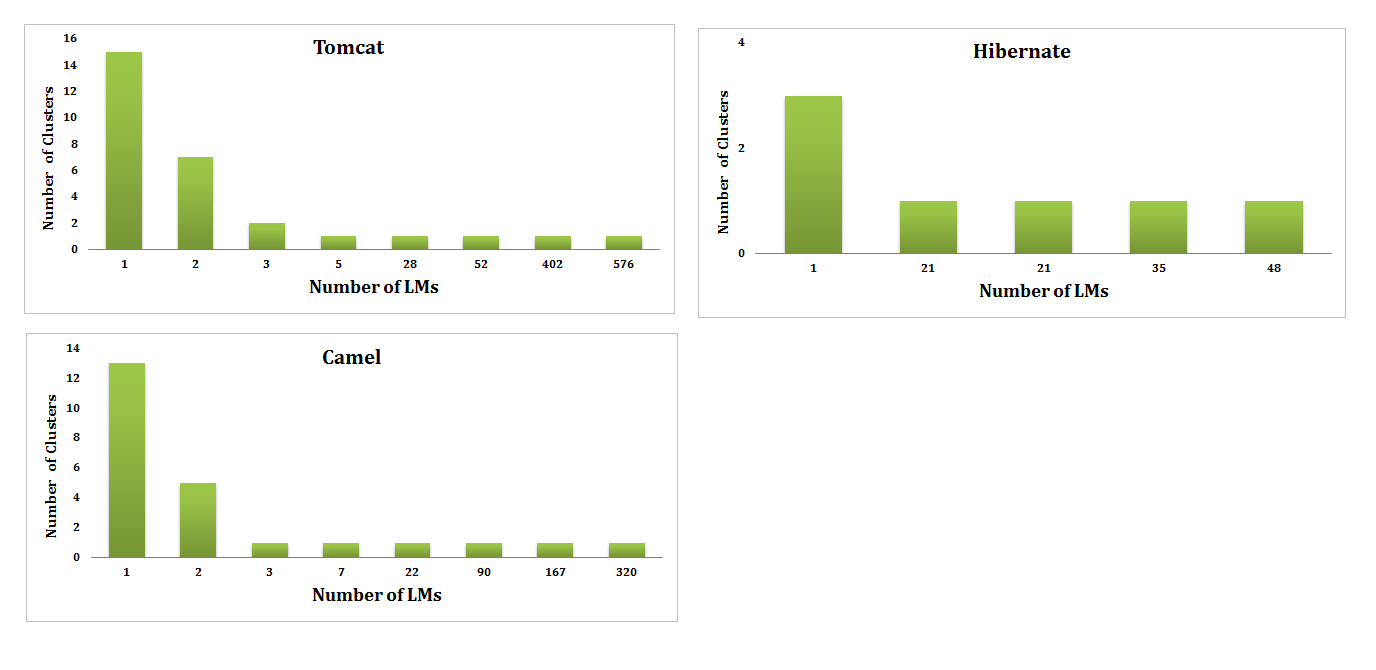
\includegraphics [width = 1\textwidth, height = 0.5\textheight] {Charts/Histograms.png}
  \caption{Histograms of the number of LMs per cluster.}
  \label{fig:histograms}
\end{sidewaysfigure}


\subsection{Analysis}  \label{analysis}
The first research question is: \emph{"Is it possible to find patterns of where log statements occur in source code?"} As shown in Table~\ref{tab_results_1}, the number of clusters has been reduced by more than 90\% in all the studied systems, indicating that developers follow some patterns for locating the log statements in source code. Furthermore, histograms depicted in Figure~\ref{fig:histograms} show that in all the studied systems, a few clusters contain a large number of LMs; however, the other clusters contain a very small number of LMs. This indicates that in these cases, developers follow a more complex or rare way of locating log statements. These exceptions might also happen due to the poor usage of logging statements in source code, which impacts the quality of the entire system negatively.

The second research question is : \emph{``What common structural characteristics do logged methods have?''}
To address this question, I manually went through the LUSs to identify the common structural characteristics of locating log statements in source code.

%a few rare exception
%ADD-> THE USAGE WITH AN EXCEPTION

\subsubsection{\emph{Categorizing logging usage}} \label{categories}
In this section, I will describe the anti-unifiers of logging usage by examining the LUSs produced by \tool{ELUS}. In general, there are five main categories of anti-unifiers in the logging usage. Each category represents one cluster of each software system that contains a large number of LMs, that is, the cluster anti-unifier represents a common way of locating log statements in source code. In the following sections, I will describe the common structural characteristics of each category represented by the anti-unifier. In addition, Figure~\ref{fig:categories} presents the number of LMs in each category and its percentage of the total number of LMs for each of the software systems. As shown in this figure, the distribution of logging categories vary from application to application, which implies that logging guidelines should be provided at application-specific level in order to establish effective logging practices.
% that their anti-unifiers are corresponded, as they have common structural characteristics. Also, these clusters
\begin{sidewaysfigure} [p]
   \centering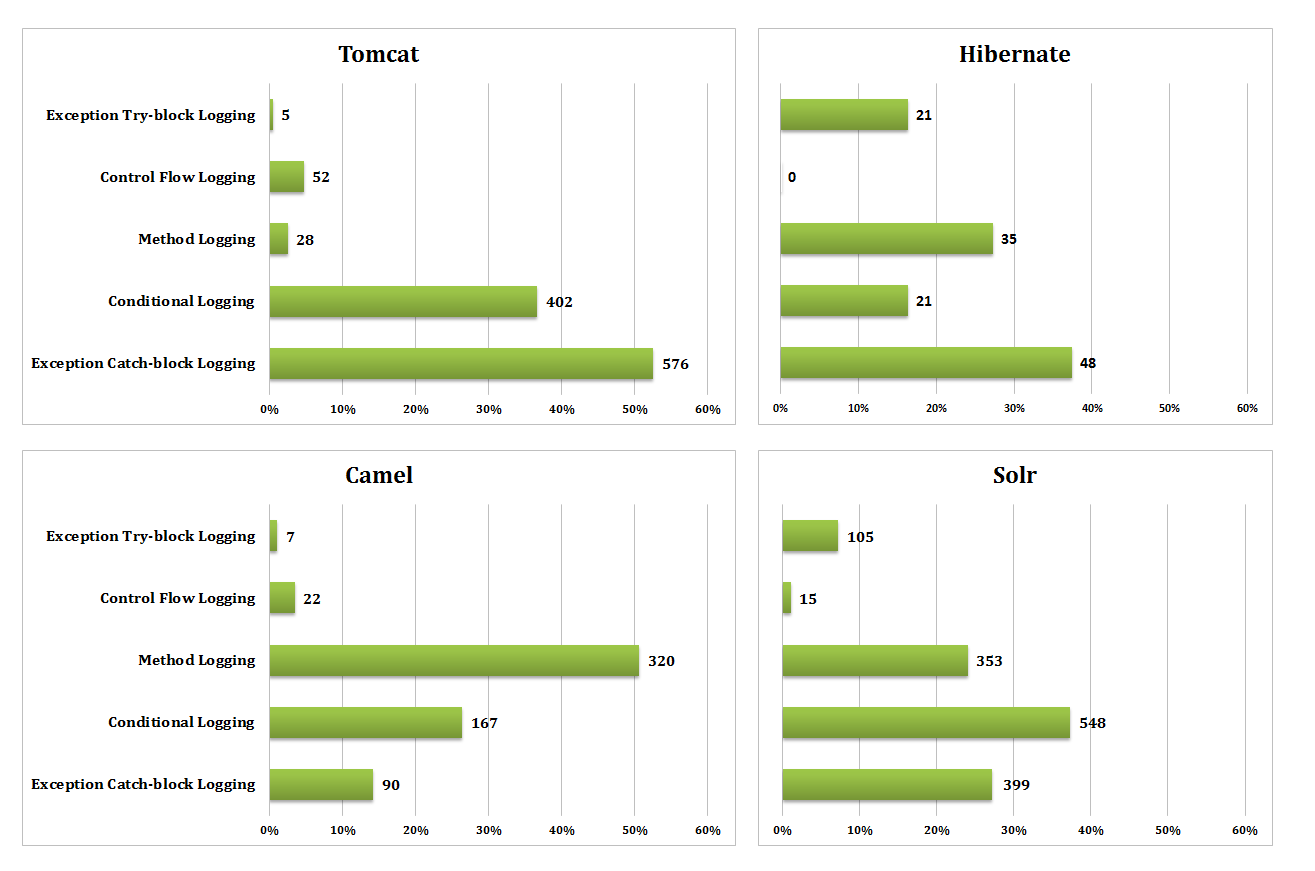
\includegraphics [width = 1\textwidth, height = 0.7\textheight]{Charts/Categories.png}
  \caption{The distribution of the categories of anti-unifiers in the logging usage.}
  \label{fig:categories}
\end{sidewaysfigure}


% how to compare?

\subsubsection{\emph{A. Exception Catch-Block Logging}}  \label{Exception catch-block logging}
The main common structural characteristics of the anti-unifiers of this category are the \code{try} statements, where the log statements are located inside the body of a \code{catch} clause. As shown in Figure~\ref{fig:categories}, 14\% to 52\% of the total LMs are described by the anti-unifiers of this category, and it is the most commonly used logging usage category in the \name{Tomcat} and \name{Hibernate} software systems. The popularity of this category among all the studied systems is due to the fact that exception handling using the \code{try}/\code{catch} blocks is a common technique in the Java programming language.

%a large portion of LMs are described by the anti-unifiers of this category.

\subsubsection{\emph{B. Conditional Logging}}  \label{conditional logging}
In this category, log statements are enclosed by \code{if}-statements with their test expressions mostly among \textit{infixExpression}, \textit{methodInvocation}, or \textit{binaryExpression} nodes. The \textit{infixExpression}s mostly either check the equality of an expression to the null literal or tests the validity of the value of a variable; the \code{if}-statements testing \textit{methodInvocation}s mostly check if the return value of an invoked method is an indicator of a potential problem within a system; and the \code{if}-statements testing \textit{binaryExpression}s mostly check if a Boolean literal is incorrect. As shown in Figure~\ref{fig:categories}, 16\% to 37\% of the total LMs are described by the anti-unifiers of this category, and it is the most commonly used logging category in the \name{Solr} system.

\subsubsection{\emph{C. Outer Method Logging}}  \label{method logging}
In this category, the log statements are located inside the body of \textit{methodDeclaration} nodes but outside of other structures nested therein. A common structural characteristic of the anti-unifiers in this category is that they mostly use the \code{throw} statement to throw an exception if an error occurs. The percentage of LMs that are described by the anti-unifiers of this category ranges from 3\% to 51\%, and it is the most common logging usage category in the \name{Camel} software system. This suggests that developers use logging to record important method granularity information about the state of a software system. This information might be used later to detect the root causes of an application problem.
% %?
% throw exception



\subsubsection{\emph{D. Control Flow Logging}}  \label{Control flow logging}
In this category, the log statements are located inside the body of either \code{switch}- or \code{if}-\code{else} statements. These log statements can be used to reveal necessary information to track the location of root causes of a potential problem in a software system. According to the Figure~\ref{fig:categories}, 0\% to 5\% of the total LMs are described by the anti-unifiers of this category.


\subsubsection{\emph{E. Exception Try-Block Logging}}  \label{Exception try-block logging}
In this category, the log statements are located inside the body of the \code{try} clause of \code{try}/\code{catch} statements. These log statements can be used to record important information about the code that may throw an exception. As shown in Figure~\ref{fig:categories}, 0\% to 7\% of the total LMs of the studied systems are described by the anti-unifiers of this category.

%COMPARE SYSTEMS???
%CATEGORIES FIGURE CHANGE???

\section{Evaluation}  \label{evaluation}
%\RW{For constrained variables, the precision should be 100\%.  The fact that it is not means that there are some bugs.  There is no point in pretending otherwise; you are better off pointing this out.  It's OK: all software contains bugs.  Later, in the Discussion, you should point out that intermediate forms of constraint are possible: instead of constraining to only the exactly desired substitutions, you can constrain to the legal types of nodes (like methodInvocation) that can be used to substitute a variable.  The (still open) question is if that would yield better results than unconstrained variables.}
%\NZ{I added it to the discussion chapter}

An empirical study is conducted to evaluate the quality of the anti-unifiers generated by \name{ELUS} in describing the location of log statements in source code. Section~\ref{precision} describes the process of evaluating the precision and recall of \tool{ELUS}.


\subsection{{Calculating the precision and recall}}  \label{precision}
To find the locations in source code that are described by an anti-unifier using \tool{ELUS}, I applied the \func{Determine-Locations} algorithm, which takes the anti-unifier and a list of all methods in source code and outputs a list of methods that their AUAST matches the anti-unifier AUAST. This algorithm anti-unifies each method in the list with the anti-unifier using the \func{Antiunify} algorithm described in Section~\ref{meth-antiUnifier} (lines~2--3). If the result equals the anti-unifier, that method will be added to the list of locations matching the anti-unifier (lines~4--5). \func{Equals} is a procedure that takes two AUAST nodes and checks whether they are equal or not. To evaluate the generalizability of the anti-unifiers, I have implemented this procedure in two ways: (1) when variables are considered to be \emph{constrained}, it tests that the non-variable nodes are identical in the two AUASTs and checks if the constraints of variable are identical or not; (2) when variables are considered to be \emph{unconstrained}, it tests that the non-variable nodes are identical in the two AUASTs, but permits unconstrained variables to differ. I ran my tool on the source code of the four studied systems and applied this algorithm to find the locations in the code that matches the structure of the generated anti-unifiers. Then, the precision and recall metrics are calculated using Equations~\ref{precision_eq} and~\ref{recall_eq}, respectively.


\begin{algorithm}
\caption{\func{Determine-Locations}($\id{antiUnifier}$,$\id{methods}$) finds the locations in source code that matches an anti-unifier.}
\label{alg-determine-locations}
\begin{algorithmic}[1]
\DetermineLocations
    \State $\id{locations} \gets \{\}$
    \For {$\id{method} \in \id{methods}$}
    \State $\id{result} \gets  \func{AntiUnify}(\id{antiUnfier}, \id{method})$
		\If {$\func{Equals}(\id{result}, \id{antiUnifier})$ }	
				 	\State{$\func{Append}(\id{method}, \id{locations})$ }
		\EndIf 		
		\EndFor
 \Return $\id{locations} $  	
  \end{algorithmic}
\end{algorithm}

\begin{equation}\label{precision_eq}
\id{precision} = \frac{\id{TP}}{{\id{TP}+\id{FP}}}
\end{equation}


\begin{equation}\label{recall_eq}
\id{recall} = \frac{\id{TP}}{{\id{TP}+\id{FN}}}
\end{equation}


Where $\id{TP}$ is the number of correct locations obtained, $\id{FP}$ is the number of incorrect locations retrieved, and $\id{FN}$ is the number of correct locations that were not retrieved. Figures~\ref{fig:precision} and \ref{fig:recall} show the precision and recall results for each software system where the experiment was run once with constrained variables and once with unconstrained variables.


\begin{figure} [H]
  \centering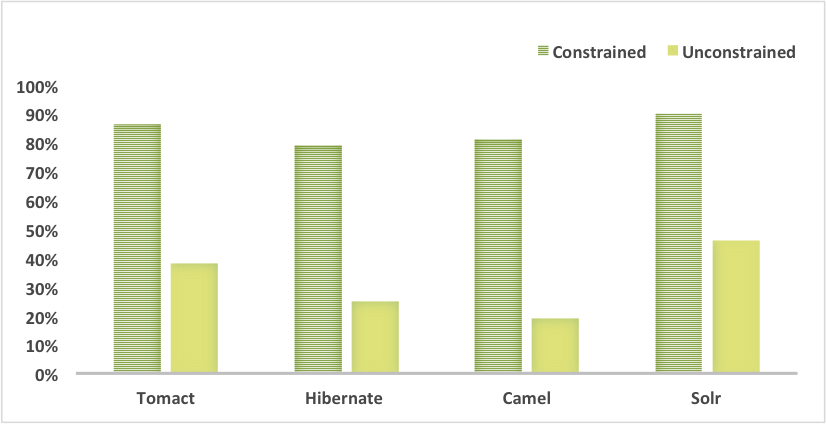
\includegraphics [width = 0.7\textwidth, height = 0.3\textheight]{Charts/Precision.png}
  \caption{The precision of \tool{ELUS}.}
  \label{fig:precision}
\end{figure}

\begin{figure} [H]
  \centering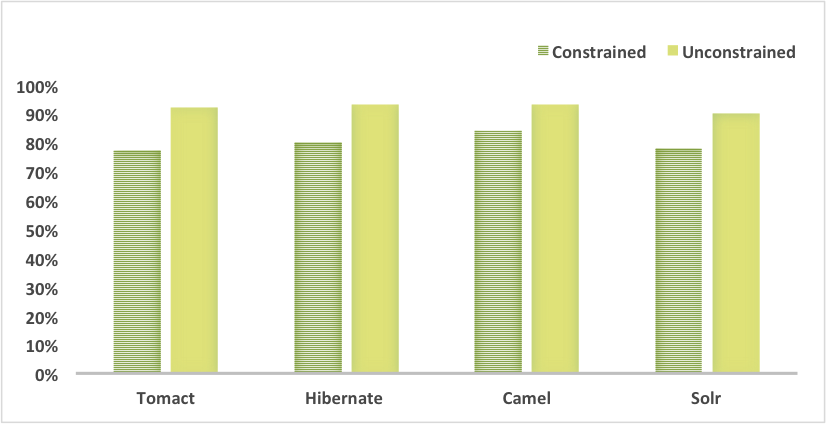
\includegraphics [width = 0.7\textwidth, height = 0.3\textheight]{Charts/Recall.png}
  \caption{The recall of \tool{ELUS}.}
  \label{fig:recall}
\end{figure}

\subsection{{Precision results}}  \label{precision-results}
The green and yellow bars in Figure~\ref{fig:precision} show the precision results when the experiment was run with constrained and unconstrained variables, respectively. I have also calculated the overall average precision of \tool{ELUS}, by averaging the precision values between the four software systems. The average precision for \tool{ELUS} is 84\% and 32\% for constrained and unconstrained variable experiments, respectively. In general, the precision for constrained variables is fairly high. The main reason behind the high precision of constrained variables is that in these cases, the variables can only be substituted with some particular nodes, which makes the anti-unifier very specific. However, there are two main reasons for the fact that precision of constrained experiment is not 100\%:
\begin{enumerate} [leftmargin=.5in]

\item \emph{Split cases}: To handle the cases containing multiple log statements, I split them into more than one case, where each contains only one logging statement (see Section~\ref{meth-multipleLogs}). However, to find the locations in source code that are described by anti-unifiers using the \func{Determine-Locations} algorithm, I compared them with all the methods in source code without splitting them into multiple cases, which results in retrieving a number of incorrect locations.

\item \emph{Software bugs}: The fact that precision results are not ideal indicates that \tool{ELUS} has some bugs. In the further work, I aim to improve these results by fixing the software bugs.
\end{enumerate}

According to the Figure~\ref{fig:precision}, the precision is fairly low for unconstrained variables. The main reason of the low precision for these cases is the fact that the unconstrained variables can be substituted by any nodes, which makes the anti-unifiers too general. As a result, the tool finds many incorrect locations the matches the anti-unifiers.





%\RW{Rewrite this according to the discussion we had in the meeting}

\subsection{{Recall results}}  \label{recall-results}
The green and yellow bars in Figure~\ref{fig:recall}  show the recall results when the experiment was run with constrained and unconstrained variables, respectively. I have also calculated the overall average recall of \tool{ELUS}, by averaging the recall values between the studied systems. The average recall for \tool{ELUS} is 80\% and 97\% for the constrained and unconstrained variable experiments, respectively. In general, when variables are constrained, \tool{ELUS} can detect many correct locations, as the recalls for all the studied systems are fairly high. Also, \tool{ELUS} can detect most of the correct locations in source code when no constraints are taken on variable nodes.

The main reason behind \tool{ELUS}'s failure to detect the correct locations is the potential complexities in constructing anti-unifiers from a large set of source code fragments. As in some cases, the anti-unifier might not maintain the correct locations of nodes in the AST hierarchy, and thus \tool{ELUS} would not be able to successfully construct the anti-unifiers of logging usage in source code.
%detect correct locations of log statements in the source code.
%?
%\RW{Ah, I see that you have a note in here about the intermediate constraints.}

%ADDDDD
% assess the generalizability of the anti-unifiers --> in between
%In general,  the tool retrieved some locations matching the anti-unifiers, while in fact they do not match.
%the tool failed to retrieve the correct locations, and in other cases



\section{Usage}  \label{usageELUS}
The insightful findings of my characterization study regarding the logging usage in several real-world software systems can be used to enhance the quality of existing logging practices by providing some logging guidelines for developers. For example, Figure~\ref{inapproprate-ex1} shows a logged method that belongs to a singleton cluster in my experiment. This \name{Java} method is an example of a poor usage of a log statement in code, as the list \code{liveNodes} can be \code{null}, and thus a \code{NullPointerException} can be thrown causing a system crash. To enhance the quality of the logging usage in this code snippet, a developer my look at our findings to be informed of how usually other developers locate log statements in similar situations. As noted in Section~\ref{categories}, to avoid the \code{NullPointerException}, developers usually insert the logging call into the body of an \code{if} statement to check if the value of the variable needed to be logged is not \code{null}. Hence, she can improve the quality of the logging usage in this example by inserting the logging call inside an \code{if} statement and log the needful information if the value of the list \code{liveNodes} is not \code{null} (lines~6--8 of Figure~\ref{approprate-ex1}). This example demonstrates how these findings can be used in practice to improve the quality of logging practices.
% in real-world application.


\begin{figure}[p]
\def\baselinestretch{1}
\begin{lstlisting}[escapechar=!]
public void setUp() throws Exception {
    SolrZkClient zkClient=new SolrZkClient(zkServer.getZkAddress(),AbstractZkTestCase.TIMEOUT);
    for (int i=0; i < 30; i++) {
       List<String> liveNodes=zkClient.getChildren("/live_nodes",null,true);
       Thread.sleep(1000);
       !\colorbox{yellowGreen}{log.info("Waiting for more nodes to come up, now: " + liveNodes.size());}!
    }
}
\end{lstlisting}
\caption[An example of an inappropriate usage of a log statement in a Java method.]{An example of an inappropriate usage of a log statement in a Java method.\label{inapproprate-ex1}}
\end{figure}



\begin{figure}[p]
\def\baselinestretch{1}
\begin{lstlisting}[escapechar=*]
public void setUp() throws Exception {
    SolrZkClient zkClient=new SolrZkClient(zkServer.getZkAddress(),AbstractZkTestCase.TIMEOUT);
    for (int i=0; i < 30; i++) {
       List<String> liveNodes=zkClient.getChildren("/live_nodes",null,true);
       Thread.sleep(1000);
       *\colorbox{yellowGreen}{if (liveNodes != null) }*
         *\colorbox{yellowGreen}{log.info("Waiting for more nodes to come up, now: " + liveNodes.size()); }*
    }
}
\end{lstlisting}
\caption[Modified Java method of Figure~\protect\ref{inapproprate-ex1} for the purpose of enhancing the logging usage.]{Modified Java method of Figure~\ref{inapproprate-ex1} for the purpose of enhancing the logging usage.\label{approprate-ex1}}
\end{figure}
   % !\colorbox{yellowGreen}{}}!
  %!\colorbox{yellowGreen}{if (liveNodes  null) { }!

\section{Summary}
I conducted an experimental study to characterize the location of log statements by applying my tool on the source code of four full software systems that make use of the \name{Apache log4j} logging framework. My tool inputs the source code of these systems, extracts ASTs of LMs, applies the proposed anti-unification and clustering algorithms, and outputs the anti-unifier for each cluster. I also conducted an experimental study to evaluate the precision and the recall of \tool{ELUS} in constructing the anti-unifiers that describe the location of log statements in source code. This experiment shows that \tool{ELUS} has achieved promising results in terms of precision and recall. Furthermore, the results taken from the characterization experiment shows that there are common ways of locating log statements. I manually examined the detailed view of structural generalizations and categorized the anti-unifiers of logging usage. In the last section of this chapter, I provided an example to demonstrate the usage of the findings of my characterization study in practice.


% In summary, this experiment shows that \tool{ELUS} has achieved promising results in terms of precision and recall metrics.

% My analysis has resulted in ... different anti-unifiers in the logging usage.

% figure out the common structural characteristics of LMs in each cluster.
%I found out that most log statements are embedded inside ....
